\documentclass{ieeeaccess}
\usepackage{cite}
\usepackage{amsmath,amssymb,amsfonts}
\usepackage{algorithmic}
\usepackage{algorithm}
\usepackage{graphicx}
\usepackage{textcomp}
\usepackage{url}
\usepackage{listings}
\usepackage{xcolor}
\usepackage[justification=centering]{caption}
\usepackage{hyperref}
% Every \cite and \ref is a clickable link to its target; every DOI/URL in the
% reference list opens the original publication.
\hypersetup{colorlinks=true, linkcolor=blue, citecolor=blue, urlcolor=blue}

\newcommand{\xmark}{\text{\sffamily X}}
\newcommand{\sep}{\,$\cdot$ }

\lstset{
  basicstyle=\ttfamily\scriptsize,
  breaklines=true,
  frame=single,
  columns=fullflexible,
  keepspaces=true,
  showstringspaces=false,
  captionpos=b
}

\usepackage{bm}
\makeatletter
\AtBeginDocument{\DeclareMathVersion{bold}
\SetSymbolFont{operators}{bold}{T1}{times}{b}{n}
\SetSymbolFont{NewLetters}{bold}{T1}{times}{b}{it}
\SetMathAlphabet{\mathrm}{bold}{T1}{times}{b}{n}
\SetMathAlphabet{\mathit}{bold}{T1}{times}{b}{it}
\SetMathAlphabet{\mathbf}{bold}{T1}{times}{b}{n}
\SetMathAlphabet{\mathtt}{bold}{OT1}{pcr}{b}{n}
\SetSymbolFont{symbols}{bold}{OMS}{cmsy}{b}{n}
\renewcommand\boldmath{\@nomath\boldmath\mathversion{bold}}}
\makeatother

\begin{document}
\history{Date of publication xxxx 00, 0000, date of current version xxxx 00, 0000.}
\doi{10.1109/ACCESS.2024.0429000}

\title{AnchorSlice: Anchor-Guided Static Slicing for Token-Efficient Smart Contract Vulnerability Detection}

\author{\uppercase{Sajad Aghanasiri}\authorrefmark{1},
\uppercase{Sina Zaker}\authorrefmark{1},
\uppercase{Alireza Shameli-Sendi}\authorrefmark{1}}

\address[1]{Faculty of Computer Science and Engineering, Shahid Beheshti University (SBU), Tehran, Iran
(e-mail: \{s.aghanasiri, a\_shameli\}@sbu.ac.ir)}

\tfootnote{This work was not supported by any specific grant but was conducted as part of academic research at Shahid Beheshti University.}

\markboth
{Aghanasiri \headeretal: AnchorSlice: Token-Efficient Smart Contract Vulnerability Detection}
{Aghanasiri \headeretal: AnchorSlice: Token-Efficient Smart Contract Vulnerability Detection}

\corresp{Corresponding author: Alireza Shameli-Sendi (e-mail: a\_shameli@sbu.ac.ir).}

\begin{abstract}
Automated vulnerability detection is a prerequisite for deploying smart contracts safely, because a deployed contract is immutable and every defect in it remains reachable by an adversary. Detectors that reason directly over source code have become increasingly capable, but their cost, latency and context capacity are bounded by the number of tokens they read, and a typical Solidity contract is dominated by comments, library code and boilerplate that cannot host a vulnerability. This paper presents AnchorSlice, a static slicing stage that makes smart contract vulnerability detection token-efficient by reducing each contract, before it reaches the detector, to the fragments capable of hosting each vulnerability category of the DASP taxonomy. AnchorSlice is purely lexical: category-specific anchor expressions and brace matching decide what survives, overlapping regions are merged once and tagged with every category they may host, and unmodified library constructs are collapsed to stubs under a rescue rule that preserves evidence. The slicer needs no compilation and processes a contract in 7.6 ms on average. On 200 contracts from the DIVE benchmark it retains 56.5\% of source characters while preserving evidence for all 463 labelled category instances, a retention of 1.00 in every category. We compare the way a source-level detector is used in practice, which is to submit the complete contract with a short instruction, against the same detector reading an AnchorSlice output with a calibrated prompt. Token consumption falls by 55.2\%, cost by 63.7\% and wall-clock time by 59.7\%, while F1-score against the benchmark rises from 0.342 to 0.693, agreement from 0.642 to 0.801 and Cohen's kappa from 0.097 to 0.549; missed vulnerabilities fall from 314 to 104 and false positives from 259 to 214 at the same time (McNemar exact test over 1,600 paired cells, $p \approx 3.7 \times 10^{-26}$). On the 130 contracts that played no part in developing the method the result is unchanged (F1-score 0.689). Token cost and detection quality therefore improve together.
\end{abstract}

\begin{keywords}
smart contract vulnerability detection, token efficiency, static slicing, input reduction, blockchain security, DASP taxonomy
\end{keywords}

\titlepgskip=-21pt

\maketitle

%============================================================
\section{Introduction}\label{sec:introduction}
%============================================================
\PARstart{D}{etecting} vulnerabilities in smart contracts before they are deployed is one of the few effective defences available on public blockchains, and detectors that read contract source code directly have become considerably more capable in recent years. Their cost, however, grows with the length of what they read, while much of a deployed contract is irrelevant to any vulnerability. This section motivates the problem of \emph{token-efficient smart contract vulnerability detection}. It first explains why contract defects are costly and why existing analysers leave the detection problem open, then shows how the input length of source-level detectors has become a limiting factor, and finally introduces AnchorSlice, summarises the contributions of this work, and poses the research questions that structure its evaluation.

Smart contracts turn contractual clauses into code that executes without a trusted intermediary~\cite{szabo1997}, and on Ethereum they hold and move assets directly~\cite{wood2014}. That property is also the problem. A contract is immutable once deployed, its bytecode is public, and any defect in it is permanently reachable by an adversary who can read the source. The 2016 DAO incident, in which a reentrancy fault drained roughly sixty million dollars, made this concrete and motivated the first generation of automated analysers~\cite{luu2016}. Practitioners subsequently organised the recurring fault patterns into the Decentralized Application Security Project (DASP) Top~10~\cite{dasp}, which remains the vocabulary against which most detection work is evaluated.

A decade of tooling has not settled the problem. When nine widely used analysers were run over 47,587 deployed contracts, they collectively identified only a minority of the annotated faults and flagged 97\% of the corpus as vulnerable, a false-positive rate that makes unattended use impractical~\cite{durieux2020}. Controlled bug injection reaches the same conclusion from the opposite direction: injected faults of well-understood shapes go undetected by tools designed specifically to find them~\cite{ghaleb2020}. The difficulty is not that analysers such as Slither~\cite{feist2019} reason poorly about control flow, but that many real defects are semantic. Whether a missing modifier matters depends on what the function does, and no fixed data-flow pattern captures that. Learning-based detectors were introduced partly to close this gap~\cite{zhuang2020}.

Detectors that reason over source code with pre-trained language models changed the trade-off again. Because such models carry general knowledge of programming idioms and security reasoning, a contract can be examined directly, without a hand-written rule for each fault class. Pipelines that pair model reasoning with static confirmation~\cite{sun2024gptscan}, that split auditing into generation and criticism~\cite{hu2023gptlens}, or that fine-tune a detector and then argue about its output through cooperating agents~\cite{ma2025iaudit} all report detection quality beyond that of pattern-based tools, and a recent systematic review counts a rapidly growing body of such work~\cite{he2024review}. In all of these systems the language model is a component of the detector rather than the object of study; what they share is that the detector consumes the contract source.

This dependence has a cost that scales with input length. A source-level detector is billed per token and bounded by a context window, and long inputs also degrade reasoning: accuracy falls when the relevant evidence sits in the middle of a long input rather than near its edges~\cite{liu2024lost}. For smart contracts the waste is easy to see. A fixed-supply ERC-20 token is several hundred lines of library boilerplate wrapped around perhaps thirty lines that could plausibly hold a flaw, yet the whole file is submitted. Prompt compression attacks the general version of this problem by using a small model to drop low-information tokens~\cite{jiang2023llmlingua}, but that approach is domain-agnostic, itself consumes model capacity, and offers no guarantee that security-relevant code survives.

We take the opposite route and exploit the fact that vulnerability classes have lexical footprints. A reentrancy fault requires an external call, a bad-randomness fault requires a block-derived value, and an arithmetic fault requires an operator. Code containing none of these cannot host the corresponding defect, and deciding that requires no model. This paper introduces AnchorSlice, a purely static slicing stage that keeps, for each DASP category, only the regions whose tokens make the category possible, and hands the detector a compact annotated slice instead of the full file. The design borrows the intuition of program slicing~\cite{weiser1981} but deliberately stops short of dependence analysis, so that the slicer runs in milliseconds and never needs to compile. It extends the candidate-pruning idea of our earlier LineGuard framework~\cite{lineguard}, which restricts the detector's view for one vulnerability category at a time, to all eight categories in a single pass with a measurable evidence guarantee. We evaluate AnchorSlice on the DIVE multi-label benchmark~\cite{dive2026}, whose 22,330 contracts are annotated for the eight DASP categories we target.

The primary contributions of this paper are summarised as follows:
\begin{itemize}
    \item We present \emph{AnchorSlice}, a detector-agnostic, purely lexical slicing stage for token-efficient smart contract vulnerability detection. It defines an anchor set for DASP categories 1--8, a visibility gate, a tag-preserving merge that emits each source region once while labelling it with every category it may host, and a library-collapse step with a rescue rule that restores lost evidence.
    \item We validate the slicer against the DIVE benchmark and show that it retains evidence for all 463 labelled category instances across 200 contracts, a retention of 1.00 in every category, while emitting 56.5\% of the original characters at an average of 7.6~ms per contract. We also report which semantic restrictions are compatible with the benchmark's annotation policy and which are not.
    \item We report a paired evaluation of the pipeline against the way such a detector is used in practice. Token consumption falls by 55.2\%, cost by 63.7\% and runtime by 59.7\%, while F1-score rises from 0.342 to 0.693 and both error types fall together, and we separate the contribution of the slice from that of the prompt, test significance, and analyse which anchors carried information and which misled the detector.
\end{itemize}

Our study is structured around the following research questions:
\begin{itemize}
    \item \textbf{RQ1 (Evidence retention):} To what extent can a purely lexical, taxonomy-anchored slice reduce the source of a smart contract while preserving the code evidence for every labelled vulnerability category?
    \item \textbf{RQ2 (Token efficiency):} How much do the token consumption, runtime and monetary cost of vulnerability detection fall when the detector receives the slice instead of the complete contract?
    \item \textbf{RQ3 (Detection effectiveness):} How does slicing affect vulnerability detection effectiveness, both in aggregate and for each DASP category?
\end{itemize}

The remainder of this paper is structured as follows. Section~\ref{sec:related} reviews previous work on smart contract vulnerability detection and input reduction. Section~\ref{sec:anchorslice} introduces AnchorSlice and its design. Section~\ref{sec:eval} presents the experimental evaluation and answers the research questions. Section~\ref{sec:limit} discusses limitations and threats to validity. Finally, Section~\ref{sec:conclusion} concludes the paper and outlines future work.

%============================================================
\section{Background and Related Work}\label{sec:related}
%============================================================
Token-efficient vulnerability detection draws on bodies of work that have rarely been considered together: analysers and detectors for smart contract vulnerabilities, techniques that reduce the input an analysis component must process, and the labelled benchmarks against which both are evaluated. This section reviews them in that order. Sections~\ref{subsec:rw_rule} to~\ref{subsec:rw_model} cover rule-based program analysis, learning-based detection, and source-level detectors built on language models, with attention to how much input each consumes. Section~\ref{subsec:rw_reduction} reviews input reduction and program slicing, Section~\ref{subsec:rw_bench} the benchmarks used for evaluation, and Section~\ref{subsec:rw_position} positions AnchorSlice against the closest prior work, as summarised in Table~\ref{tab:related_work}.

\begin{table*}[htbp]
\centering
\caption{Positioning of AnchorSlice Against Prior Work on Vulnerability Detection and Input Reduction}
\label{tab:related_work}
\footnotesize
\renewcommand{\arraystretch}{1.15}
\resizebox{\textwidth}{!}{%
\begin{tabular}{l c l l l c c}
\hline
\textbf{Work} & \textbf{Year} & \textbf{Technique} & \textbf{Input to the detector} & \textbf{Input reduction} & \textbf{Model-free reduction} & \textbf{Taxonomy-guided} \\
\hline
\cite{luu2016} Oyente & 2016 & Symbolic execution & EVM bytecode & None & -- & -- \\
\cite{tsankov2018} Securify & 2018 & Dependence-graph patterns & EVM bytecode & None & -- & -- \\
\cite{tikhomirov2018} SmartCheck & 2018 & XML-based patterns & Solidity source & None & -- & -- \\
\cite{feist2019} Slither & 2019 & SSA-based static analysis & Solidity source & None & -- & -- \\
\cite{li2018vuldeepecker} VulDeePecker & 2018 & Deep learning & Code gadgets & Slicing around API calls & \checkmark & \xmark \\
\cite{li2022sysevr} SySeVR & 2022 & Deep learning & Semantic slices & Dependence-based slicing & \checkmark & \xmark \\
\cite{zhuang2020} Zhuang et al. & 2020 & Graph neural network & Contract graph & Graph normalisation & \checkmark & \xmark \\
\cite{sridharan2007} Thin slicing & 2007 & Program slicing & Program & Value-flow slicing & \checkmark & \xmark \\
\cite{jiang2023llmlingua} LLMLingua & 2023 & Prompt compression & Compressed prompt & Small-model token dropping & \xmark & \xmark \\
\cite{jiang2024longllmlingua} LongLLMLingua & 2024 & Prompt compression & Compressed prompt & Question-aware token dropping & \xmark & \xmark \\
\cite{lineguard} LineGuard & 2025 & Model-based line localisation & Pruned candidate lines & Per-category regex pruning & \checkmark & Single category \\
\textbf{AnchorSlice} & 2026 & Anchor-guided static slicing & Tagged multi-category slice & Anchored windows, library collapse & \checkmark & \checkmark \\
\hline
\end{tabular}%
}
\end{table*}

\subsection{Rule-Based Security Analysis}\label{subsec:rw_rule}
Oyente introduced symbolic execution of EVM bytecode and defined several of the fault patterns still in use~\cite{luu2016}. Securify derived compliance and violation patterns from dependence graphs to make its verdicts explainable~\cite{tsankov2018}, while SmartCheck worked on an intermediate XML representation of Solidity to keep analysis lightweight~\cite{tikhomirov2018}. Mythril combined symbolic execution with taint analysis over bytecode~\cite{mythril}, and MAIAN targeted trace-level properties such as contracts that can be made to leak or lock funds~\cite{nikolic2018}. VeriSmart pushed precision further for arithmetic safety by inferring transaction invariants~\cite{so2020}. Dynamic approaches complement these: ContractFuzzer generated transaction sequences against an instrumented EVM~\cite{jiang2018contractfuzzer}, and sFuzz added an adaptive strategy for branches that random input rarely reaches~\cite{nguyen2020sfuzz}. Slither occupies a middle ground, converting Solidity to an SSA-based intermediate form that supports fast detectors and code-review aids~\cite{feist2019}. The large-scale comparisons of these tools~\cite{durieux2020} and the injection studies that probe them~\cite{ghaleb2020} both conclude that coverage remains partial and precision low, which is the gap learning-based and model-based detectors have tried to close. Because rule-based tools execute fixed analyses rather than reading tokens, input length is not their bottleneck; it becomes one only for the detectors reviewed next.

\subsection{Learning-Based Vulnerability Detection}\label{subsec:rw_learning}
VulDeePecker showed that vulnerability detection could be learned from code gadgets, slices of semantically related statements gathered around library and API calls~\cite{li2018vuldeepecker}. SySeVR generalised the idea to four syntactic seed types and used program dependence graphs for slicing~\cite{li2022sysevr}. Devign moved to graph representations that combine abstract syntax, control flow and data flow~\cite{zhou2019devign}, and LineVul demonstrated that transformer models can localise predictions to individual lines~\cite{fu2022linevul}, often building on code-specific pre-training such as CodeBERT~\cite{feng2020codebert}. In the contract setting, Zhuang et al. represented functions as normalised graphs and applied a degree-free graph convolutional network and a temporal message propagation network~\cite{zhuang2020}; later work combined such graph models with expert-designed patterns to improve interpretability~\cite{liu2023combining}. AnchorSlice is related to this literature mainly through the seed-and-expand idea: like VulDeePecker and SySeVR it begins from syntactic anchors, but it produces a reduced source for a general-purpose detector rather than a feature vector for a trained classifier, and it therefore needs no dependence graph.

\subsection{Language-Model Detectors and Their Input Cost}\label{subsec:rw_model}
Code-trained models~\cite{chen2021codex}, together with in-context learning~\cite{brown2020} and chain-of-thought prompting~\cite{wei2022cot}, made it practical to obtain a security judgement from a general model. GPTScan uses model reasoning to nominate candidate variables and statements and dedicated static modules to validate them, reporting recall above 70\% on ground-truth logic bugs~\cite{sun2024gptscan}. GPTLens splits the task between an auditor role that proposes vulnerabilities and a critic role that scores them, which suppresses over-reporting~\cite{hu2023gptlens}. LLM4Vuln decouples the components of vulnerability reasoning so that knowledge retrieval, tool use and reasoning can be measured separately~\cite{sun2024llm4vuln}. LLM-SmartAudit organises multiple agents around a conversation about the contract~\cite{wei2024smartaudit}, and Smart-LLaMA post-trains an open model in two stages to produce both a decision and an explanation~\cite{yu2024smartllama}. iAudit fine-tunes a detector and a reasoner and then has ranker and critic agents debate the cause, reaching an F1-score of 91.21\% on a curated set of 263 vulnerabilities~\cite{ma2025iaudit}. PropertyGPT goes further and generates formal properties for verification rather than verdicts alone~\cite{liu2025propertygpt}. What these detectors share is the assumption that they receive the contract, and the systematic review of the area identifies context length as a recurring constraint~\cite{he2024review}. Our earlier framework, LineGuard~\cite{lineguard}, already narrows the detector's view: for a vulnerability category given in advance, it ranks candidate lines with category-specific regular expressions and passes the top-ranked candidates with a fixed context window. That pruning serves line-level localisation of one category per query, and its effect on evidence retention and token cost was not isolated. AnchorSlice is orthogonal to all of these detectors, since any of them could consume a sliced contract instead of a whole one.

\subsection{Input Reduction and Program Slicing}\label{subsec:rw_reduction}
The cost of long inputs has been attacked generically. LLMLingua uses a small language model to identify and drop low-information tokens, reporting high compression with limited loss~\cite{jiang2023llmlingua}, and LongLLMLingua adds question-aware reordering for long-context settings~\cite{jiang2024longllmlingua}. Retrieval-augmented generation avoids the problem by fetching only relevant passages~\cite{lewis2020rag}. These methods estimate relevance statistically and therefore cannot promise that a particular security-critical line survives. Classical program slicing offers the opposite guarantee, computing the statements that can affect a criterion~\cite{weiser1981}, and thin slicing restricts the result to statements that produce the value of interest~\cite{sridharan2007}. Full slicing needs a compilable program and a dependence graph, which is a strong requirement for a corpus of deployed contracts spanning many compiler versions. AnchorSlice sits between these positions: it is coarser than dependence-based slicing, but its slicing criterion is the vulnerability taxonomy itself, and its evidence retention against a labelled benchmark can be measured directly.

\subsection{Labelled Benchmarks}\label{subsec:rw_bench}
Evaluation in this area depends on the quality of labels. ScrawlD labelled real contracts by majority vote over five analysers~\cite{yashavant2022}, and DAppSCAN built large source and bytecode datasets from 1,199 audit reports covering 682 DApp projects~\cite{zheng2024dappscan}. We use DIVE~\cite{dive2026}, which annotates 22,330 contracts deployed between 2016 and 2024 against the eight DASP categories. DIVE aggregates MAIAN, Mythril, Semgrep, Slither, Solhint and VeriSmart through a power-based voting scheme and then re-checks positive findings against category-specific code evidence, a post-hoc validation that corrected about 14.3\% of DoS and 24.9\% of time-manipulation labels. Labels are assigned at contract level, which shapes how evidence retention can be validated.

\subsection{Positioning of AnchorSlice}\label{subsec:rw_position}
Table~\ref{tab:related_work} contrasts AnchorSlice with the closest prior work along the dimensions that matter for token-efficient detection. Rule-based analysers do not reduce their input because they do not read tokens. Learning-based detectors reduce input through slicing or graph construction, but their reduction is tied to a trained representation rather than to a vulnerability taxonomy. Prompt-compression methods reduce input for token-bound models but use a model to decide what to keep and offer no guarantee for security-relevant code. LineGuard prunes with category-specific rules but for one category at a time. AnchorSlice is, to our knowledge, the first reduction stage that is simultaneously model-free, guided by the full vulnerability taxonomy, and validated for evidence retention on a labelled smart contract benchmark.

%============================================================
\section{AnchorSlice}\label{sec:anchorslice}
%============================================================
AnchorSlice turns a complete Solidity contract into a compact, annotated slice that retains, for every DASP category, the code regions able to host that category, so that a downstream vulnerability detector reads fewer tokens without losing the evidence it needs. Fig.~\ref{fig:pipeline} places the slicer in the detection pipeline, and Algorithm~\ref{alg:anchorslice} gives the complete procedure, which runs in three stages: comment removal, library collapse, and anchor-guided window extraction. This section first states the principles that constrain the design (Section~\ref{subsec:design}), then describes the lexical anchors and the single semantic gate retained (Section~\ref{subsec:anchors}), the extraction and tag-preserving merge of windows (Section~\ref{subsec:merge}), library collapse and its evidence rescue rule (Section~\ref{subsec:rescue}), and finally how the slice is rendered and handed to the detector (Section~\ref{subsec:render}).

\begin{figure*}[htbp]
    \centering
    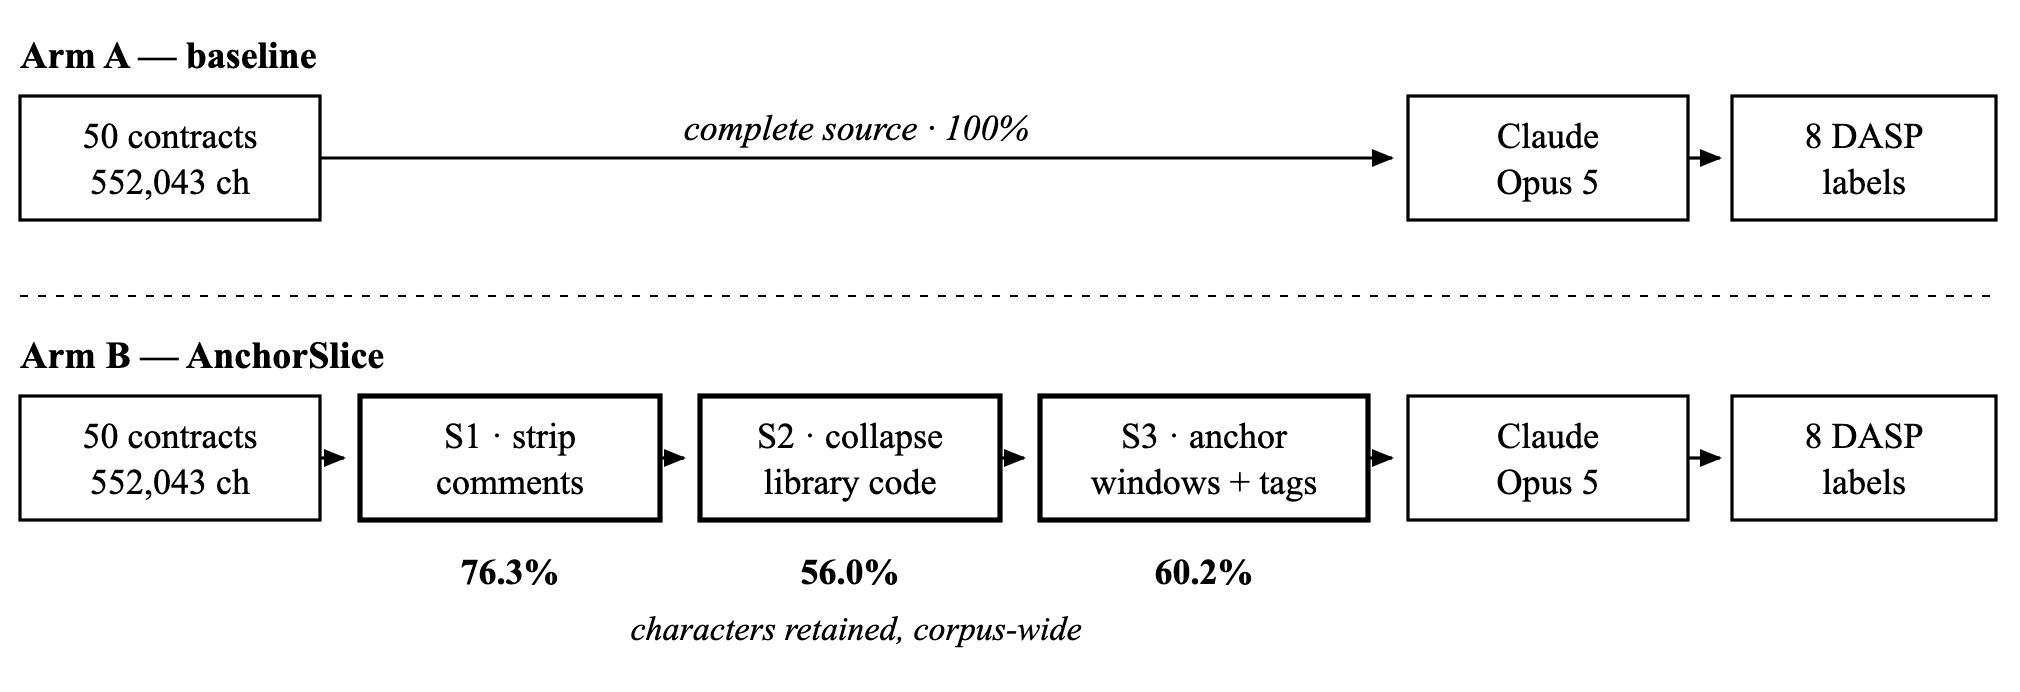
\includegraphics[width=\linewidth, keepaspectratio]{fig1_pipeline.png}
    \caption{The two arms of the experiment on 200 contracts. Arm~A is ordinary practice: the complete source is submitted with a short instruction. Arm~B inserts the three AnchorSlice stages S1--S3 and pairs the slice with the calibrated prompt. The detector, Claude Opus~5, and the output schema are identical in both arms; the per-contract cost of each arm is given beneath it.}
    \label{fig:pipeline}
\end{figure*}

\begin{algorithm}[t]
\caption{AnchorSlice}
\label{alg:anchorslice}
\begin{algorithmic}[1]
\REQUIRE Source $S$, categories $\mathcal{C}$ with anchors $\{A_c\}$, gated set $\mathcal{V}\subseteq\mathcal{C}$, cap $\kappa$, padding $\pi$
\ENSURE Annotated slice $\Sigma$
\STATE $L \leftarrow$ \textsc{StripComments}$(S)$
\STATE $K \leftarrow$ lines of top-level library units in $L$ \COMMENT{collapsed}
\STATE $W \leftarrow \emptyset$
\FOR{each function $f=(f_s,f_e,\textit{sig})$ in $L$ with $f_s \notin K$}
    \STATE $G \leftarrow \mathcal{V}$ \textbf{if} \textit{sig} is \texttt{view}/\texttt{pure} \textbf{else} $\emptyset$
    \FOR{$k = f_s$ \TO $f_e$}
        \STATE $T \leftarrow \{\, c \in \mathcal{C}\setminus G : A_c \text{ matches } L[k] \,\}$
        \IF{$T \neq \emptyset$}
            \STATE $(a,b) \leftarrow$ \textsc{InnermostBlock}$(L,f,k,\kappa,\pi)$
            \STATE $W \leftarrow W \cup \{(a,b,T)\}$
        \ENDIF
    \ENDFOR
\ENDFOR
\STATE $B \leftarrow$ \textsc{MergeAdjacent}$(W)$ \COMMENT{union of tags}
\FOR{each $c \in \mathcal{C}$ tagged in no block of $B$}
    \IF{some $k \in K$ has $A_c$ matching $L[k]$}
        \STATE $B \leftarrow B \cup \{(k-1,k+1,\{c\})\}$ \COMMENT{rescue}
    \ENDIF
\ENDFOR
\STATE $\Sigma \leftarrow$ \textsc{Render}$(\text{stubs}(K), \text{declarations}(L), B)$
\IF{$|\Sigma| \geq |L|$}
    \STATE $\Sigma \leftarrow L$ \COMMENT{small contract: send whole}
\ENDIF
\STATE \textbf{return} $\Sigma$
\end{algorithmic}
\end{algorithm}

\subsection{Design Principles}\label{subsec:design}
Three requirements shaped the design. First, the slicer must be fully static, in the sense that every decision follows from regular expressions and brace counting; a slicer that needed model judgement to decide what to keep would spend the token budget it is meant to save. Second, it must emit each region of source at most once. Running eight independent category-specific passes would be the obvious construction, but the passes overlap heavily and their union would exceed the original file, so AnchorSlice performs a single pass and attaches a set of candidate categories to each emitted region (Algorithm~\ref{alg:anchorslice}, lines~4--14). Third, the slicer must be detector-agnostic: its output is ordinary Solidity text with comment headers, so any source-level detector can consume it without modification.

\subsection{Lexical Anchors and the Visibility Gate}\label{subsec:anchors}
Each category owns a set of anchor expressions, and a line matching one marks its enclosing region as a candidate for that category (line~7). Two macros carry most of the weight. \texttt{EXT} matches any external or cross-contract call, including low-level \texttt{call}, \texttt{send}, \texttt{transfer}, \texttt{delegatecall} and \texttt{staticcall} forms, calls through an interface cast, and calls on a receiver that is not a language builtin. \texttt{MUTFN} matches any public or external function that is not declared \texttt{view} or \texttt{pure}. The second macro deserves comment. Access-control faults are often an absence rather than a presence, so no positive pattern can find them; treating every state-mutating entry point as a candidate is the only static way to surface a contract whose fault is a missing modifier.

We evaluated five semantic gates intended to suppress obviously safe regions and retained one. Suppressing arithmetic candidates in contracts compiled under Solidity 0.8, where overflow reverts by default, cut arithmetic recall from 1.00 to 0.43, because DIVE labels many such contracts positive regardless. Requiring a state write before admitting a reentrancy candidate cut its recall from 0.91 to 0.36. Treating a call wrapped in \texttt{require} as a checked return cut that category from 0.60 to 0.20. Only the visibility gate survived: a \texttt{view} or \texttt{pure} body cannot mutate state, and excluding such bodies from the five state-dependent categories cost no recall at all (line~5). The rejected gates were sound as Solidity reasoning but disagreed with the benchmark's annotation policy, which is a useful reminder that a slicer tuned to a dataset inherits that dataset's conventions. Table~\ref{tab:anchors} gives the complete anchor set, the gate applied to each category, and the evidence retention the resulting slicer achieves.

\begin{table*}[htbp]
\centering
\caption{Anchor Specification for the Eight DASP Categories}
\label{tab:anchors}
\footnotesize
\renewcommand{\arraystretch}{1.2}
\begin{tabular}{@{}p{3.1cm} p{11.1cm} c c@{}}
\hline
\textbf{Category} & \textbf{Anchor expressions} & \textbf{Gate} & \textbf{Retained} \\
\hline
Reentrancy & \texttt{EXT} & view/pure & 98/98 \\
Access Control & \texttt{modifier}\sep\texttt{only\textbackslash w+}\sep\texttt{(\_)owner =}\sep\texttt{tx.origin}\sep\texttt{selfdestruct}\sep\texttt{suicide}\sep\texttt{delegatecall}\sep\texttt{require(msg.sender}\sep\texttt{renounce}\sep\texttt{transferOwnership}\sep\texttt{authoriz}\sep\texttt{admin}\sep\texttt{MUTFN} & view/pure & 144/144 \\
Arithmetic & \texttt{[+ - * / \%]=}\sep\texttt{++}\sep\texttt{-{}-}\sep\texttt{x [+ * / \%] y}\sep\texttt{x - y}\sep\texttt{**}\sep\texttt{<{}<}\sep\texttt{>{}>}\sep\texttt{unchecked} & -- & 84/84 \\
Unchecked Return Values & \texttt{EXT} & view/pure & 38/38 \\
DoS & \texttt{for(}\sep\texttt{while(}\sep\texttt{.push(}\sep\texttt{.length}\sep\texttt{require(}\sep\texttt{revert}\sep\texttt{assert(}\sep\texttt{EXT} & view/pure & 26/26 \\
Bad Randomness & \texttt{blockhash}\sep\texttt{block.\{difficulty, coinbase, gaslimit, number, timestamp, prevrandao\}}\sep\texttt{now}\sep\texttt{keccak256}\sep\texttt{sha3(}\sep\texttt{sha256}\sep\texttt{random}\sep\texttt{nonce}\sep\texttt{seed} & -- & 16/16 \\
Front Running & \texttt{approve(}\sep\texttt{allowance}\sep\texttt{msg.value}\sep\texttt{tx.gasprice}\sep\texttt{price}\sep\texttt{bid}\sep\texttt{swap*(}\sep\texttt{slippage}\sep\texttt{amountOutMin}\sep\texttt{deadline}\sep\texttt{reserve}\sep\texttt{MUTFN} & view/pure & 15/15 \\
Time manipulation & \texttt{now}\sep\texttt{block.timestamp}\sep\texttt{block.number}\sep\texttt{N \{days, hours, minutes, seconds, weeks\}}\sep\texttt{deadline}\sep\texttt{startTime}\sep\texttt{endTime}\sep\texttt{cooldown}\sep\texttt{lastClaim}\sep\texttt{timeout} & -- & 42/42 \\
\hline
\textbf{All categories} & -- & -- & \textbf{463/463} \\
\hline
\multicolumn{4}{@{}p{17.4cm}@{}}{\scriptsize \texttt{EXT} matches low-level calls (\texttt{.call}, \texttt{.call.value}, \texttt{.send}, \texttt{.transfer}, \texttt{delegatecall}, \texttt{staticcall}), calls through an interface cast, \texttt{transferFrom}/\texttt{\_transfer}, swap and add-liquidity calls, \texttt{payable(} conversions, inline \texttt{assembly}, and calls on any receiver that is not a language builtin. \texttt{MUTFN} matches any public or external function not declared \texttt{view} or \texttt{pure}. The gate column names the only semantic restriction retained after ablation. \emph{Retained} counts the label-positive contracts that keep at least one block tagged with the category.} \\
\end{tabular}
\end{table*}

\subsection{Window Extraction and Tag-Preserving Merge}\label{subsec:merge}
An anchored line is expanded to the innermost brace block that contains it, capped at $\kappa = 10$ lines; past that cap the window falls back to the anchor with $\pi = 2$ lines of context on each side (line~9). The enclosing function signature is attached separately so that visibility and modifiers stay visible even when the body is truncated. Windows are then sorted and merged: any two whose ranges overlap or abut become a single block whose tag set is the union of theirs (line~14). A region relevant to both reentrancy and arithmetic is consequently emitted once and carries both labels, which preserves the single-emission principle. Across the evaluation corpus this produces 16.6 blocks per contract.

\subsection{Library Collapse and Evidence Rescue}\label{subsec:rescue}
Unmodified reference implementations account for a large share of a typical file. AnchorSlice detects top-level \texttt{SafeMath}, \texttt{Address}, \texttt{Context}, \texttt{Ownable}, \texttt{ERC20} and common exchange interfaces by name and replaces each with a one-line stub, so the detector still knows the construct is present (line~2). Applied naively, this cost recall, dropping access control to 0.95 and DoS to 0.86, because in a few contracts the only anchor for a category lay inside a collapsed construct. A rescue pass repairs the loss: if a category ends the pass with no block anywhere in the file while an anchor for it exists inside collapsed text, a three-line window is emitted at that anchor (lines~15--19). The rescue restores recall to 1.00 at a cost of about two percentage points of size.

\subsection{Slice Rendering and Detector Interface}\label{subsec:render}
The emitted slice begins with the stubs for collapsed libraries and the contract-level declarations, then lists the blocks in source order (line~20). Each block carries a header naming its original line range and its candidate categories, and line numbers refer to the original file so that a finding can be traced back. Fig.~\ref{fig:slice_example} shows an excerpt of the slice produced for a contract from the evaluation sample. The header reports that 61 of 128 source lines were kept in five blocks, and \texttt{SafeMath} is reduced to a stub. Block~2 is a modifier tagged for access control because it constrains \texttt{msg.sender} and for DoS because it contains \texttt{require}; block~3 is a public constructor-style function tagged by \texttt{MUTFN} for access control and front running. A short preamble tells the detector that these tags are lexical hints rather than findings and that most tagged blocks are not vulnerable. A guard handles small files: when the block headers would cost more than the removed lines save, the contract is sent whole with comments stripped (lines~21--23), which occurred for 43 of the 200 contracts in our sample.

\begin{figure}[htbp]
\centering
\begin{lstlisting}
// SLICED CONTRACT 19288: 128 src lines -> 61 kept (48%), 5 candidate blocks.
// Each block lists the DASP categories whose static anchors fired inside it.
// Omitted code matched no anchor for any category.
// [standard SafeMath omitted - unmodified reference implementation]
// --- DECLARATIONS ---
pragma solidity ^0.4.18;
[...]
// --- BLOCK 2 | src L16-21 | candidates: Access Control, DoS
    modifier onlyCLevel() {
    require(
      msg.sender == ceoAddress
    );
    _;
    }

// --- BLOCK 3 | src L23-26 | candidates: Access Control, Front Running
    function AdPotato() public{
        ceoAddress=msg.sender;
        initialize(0x58AFF91f5b48245Bd83deeB2C7d31875f68b3f0D);
    }
[...]
\end{lstlisting}
\caption{Excerpt of the AnchorSlice output for DIVE contract 19288. Lines marked \texttt{[...]} are elided here for space; all other lines are reproduced verbatim.}
\label{fig:slice_example}
\end{figure}

%============================================================
\section{Experimental Evaluation}\label{sec:eval}
%============================================================
This section evaluates whether AnchorSlice makes smart contract vulnerability detection more token-efficient without degrading it. The evaluation holds the detector fixed and changes only its input, comparing the complete contract (Arm~A) with the AnchorSlice output (Arm~B) on the same contracts. Section~\ref{subsec:setup} describes the experimental setup and configuration, Section~\ref{subsec:dataset} the dataset and sampling procedure, and Section~\ref{subsec:protocol} the evaluation protocol and metrics. Sections~\ref{subsec:retention} to~\ref{subsec:percat} report evidence retention, token consumption and runtime, detection effectiveness, and per-category behaviour. Section~\ref{subsec:discussion} revisits the research questions posed in Section~\ref{sec:introduction}.

\subsection{Setup}\label{subsec:setup}
AnchorSlice and the evaluation harness are implemented in Python using only the standard library, and the complete source, sample definitions, raw results and run logs are available in the project repository~\cite{anchorslice_repo}. The exact slicer used for the reported runs is archived there unchanged, alongside a later revision that adds guards for contract shapes this sample does not contain. Slicer runtime was measured on an Intel Core i9-9880H processor with Python~3.12.3. The detector in both arms is Claude Opus~5 at high reasoning effort, accessed through the Claude Code command-line interface in non-interactive print mode. All built-in tools and external tool servers are disabled and no session state is persisted, so the detector sees nothing beyond the prompt and cannot retrieve the answer from elsewhere. A JSON schema constrains every reply to eight binary labels with a confidence and a short justification per category, which removes output parsing as a source of error. Each contract receives a single call, calls are issued sequentially, and the interface reports token usage, latency and cost for every call. The interface does not expose sampling parameters such as temperature, so the results are reproducible in configuration and in the logged per-call record but not bit-for-bit. Table~\ref{tab:config} lists every parameter used; all of them are held fixed across both arms.

\begin{table}[t]
\centering
\caption{Experimental Configuration and Parameters}
\label{tab:config}
\footnotesize
\renewcommand{\arraystretch}{1.2}
\begin{tabular}{@{}p{2.35cm} p{1.55cm} p{3.75cm}@{}}
\hline
\textbf{Parameter} & \textbf{Value} & \textbf{Description} \\
\hline\hline
\multicolumn{3}{@{}l}{\textit{Slicer}} \\
\hline
Window cap $\kappa$ & 10 lines & Largest brace block kept whole \\
Padding $\pi$ & $\pm$2 lines & Context around an anchor past the cap \\
Gated categories $\mathcal{V}$ & 5 & Skipped inside \texttt{view}/\texttt{pure} bodies \\
\hline
\multicolumn{3}{@{}l}{\textit{Sampling}} \\
\hline
Sample size & 200 & Seeded stratified sample, three rounds \\
Category floor & 5 & Minimum positives and negatives per category \\
Size filter & 1.2--30 kB & Excludes empty stubs, bounds per-call cost \\
\hline
\multicolumn{3}{@{}l}{\textit{Detector}} \\
\hline
Model & Opus 5 & Claude Opus~5, high reasoning effort \\
Access & Claude CLI & Print mode, tools and tool servers disabled \\
Output & JSON schema & 8 binary labels, confidences, reasons \\
System prompt & calibrated & Category definitions with examples and decision-threshold guidance \\
Calls & 1 per contract & Sequential, 900 s timeout \\
Sampling & not exposed & Temperature and top-p not user-controllable \\
\hline
\end{tabular}
\end{table}

\subsection{Dataset and Sampling}\label{subsec:dataset}
We drew 200 contracts from DIVE~\cite{dive2026} with seeded random sampling, repaired so that every category carries enough positive and negative instances to be measurable in both directions; a sample composed only of heavily labelled contracts would leave precision undefined, because a detector answering all-positive would score perfectly. Contracts smaller than 1,200 bytes were excluded as empty stubs, and contracts larger than 30,000 bytes were excluded to bound the cost of each call. The sample totals 2,311,110 characters and no contract required truncation. The 1,600 label cells (200 contracts $\times$ 8 categories) contain 463 positives, a positive rate of 28.9\%. Per-category rates track the corpus closely for the common categories -- access control 72.0\% against 74.9\% corpus-wide, reentrancy 49.0\% against 51.1\% and arithmetic 42.0\% against 42.7\% -- while the two rarest categories are deliberately over-sampled, bad randomness at 8.0\% against 2.8\% and front running at 7.5\% against 2.7\%, so that they carry enough positives to be scored at all. The sample was drawn in three rounds; the 130 contracts of the last round were never inspected while the method was developed and are reported separately in Section~\ref{subsec:effectiveness}.

\subsection{Evaluation Protocol}\label{subsec:protocol}
Arm~A is the way a source-level detector is used in practice: the complete contract is submitted with a short instruction that names the eight categories in one line each and asks the detector to report a fault where it is reachable and exploitable. Arm~B is the proposed pipeline: the AnchorSlice output, preceded by a short preamble explaining the block format and stating that the category tags are lexical hints rather than findings, together with a calibrated prompt that gives each category a minimal code example, a decision rule aligned with the benchmark's annotation policy, and the corpus base rate of that category. The detector, reasoning effort, output schema and contracts are identical, with one call each. Because both arms classify the same 1,600 cells, the comparison is paired, and we report McNemar's exact test on discordant cells alongside the aggregate measures. To separate the two changes, Section~\ref{subsec:effectiveness} also compares the slice against the complete source under one fixed prompt.

We report label agreement over all cells, Hamming loss, exact match at contract level, and micro-averaged precision, recall and F1-score. Because the label distribution is unbalanced, we also report Cohen's kappa, which corrects for agreement expected by chance. Resource use is measured as total tokens across all token classes, wall-clock time, and cost. Evidence retention is measured without the detector, as the share of label-positive contracts that keep at least one block tagged with the corresponding category. All detection metrics use the DIVE labels as the reference.

\subsection{Evidence Retention and Slice Compactness}\label{subsec:retention}
AnchorSlice reduced the sample from 2,311,110 to 1,305,860 characters, or 56.5\% of the original. Evidence retention was 1.00 for every category: all 463 label-positive category instances kept at least one block tagged with that category, as summarised in Table~\ref{tab:anchors}. Reaching full retention required four guards that a smaller sample had not exercised: legacy contracts in which a function without a visibility keyword is public by default, function signatures spanning several lines, anonymous fallback functions, and minified sources in which an entire contract occupies one or two lines. A contract for which no candidate block can be isolated, or whose block headers would cost more than the removed lines save, is sent whole with comments stripped, which occurred for 43 of the 200 contracts. Decomposing the pipeline in Fig.~\ref{fig:pipeline} shows that comment removal and library collapse deliver most of the reduction, with the anchoring stage adding its block headers back. The slicer processes a contract in 7.6~ms on average and 17.5~ms at most, which is negligible beside the tens of seconds a detector call takes.

\subsection{Token Consumption, Runtime and Cost}\label{subsec:cost}
Table~\ref{tab:resources} and Fig.~\ref{fig:resources} report resource use. The pipeline cut total token consumption from 2,092,914 to 937,754, a reduction of 55.2\%, and mean consumption per contract from 10,465 to 4,689 tokens. The contract text the detector must read, measured as the tokens written to the prompt cache, fell by 69.1\%. Wall-clock time fell from 4,151 to 1,673 seconds, or 59.7\%, and cost from \$17.75 to \$6.45, a reduction of 63.7\%: \$0.032 and 8.4 seconds per contract against \$0.089 and 20.8 seconds. Output tokens fell by 55.9\% as well, because given a compact, tagged input the detector writes shorter justifications. The calibrated prompt adds roughly 1,600 tokens per call, but it is cached across calls and is far smaller than what the slice removes from the contract itself.

\begin{table}[t]
\centering
\caption{Resource Consumption Across 200 Contracts}
\label{tab:resources}
\footnotesize
\renewcommand{\arraystretch}{1.2}
\begin{tabular}{@{}l r r r@{}}
\hline
\textbf{Measure} & \textbf{Arm A} & \textbf{Arm B} & \textbf{Change} \\
\hline\hline
Input tokens & 1,837,975 & 825,285 & $-$55.1\% \\
Output tokens & 254,939 & 112,469 & $-$55.9\% \\
Contract text cached & 1,100,024 & 339,432 & $-$69.1\% \\
Cost per contract & \$0.089 & \$0.032 & $-$63.7\% \\
\textbf{Total tokens} & \textbf{2,092,914} & \textbf{937,754} & \textbf{\textminus55.2\%} \\
Tokens per contract & 10,465 & 4,689 & $-$55.2\% \\
Wall clock (s) & 4,151 & 1,673 & $-$59.7\% \\
Seconds per contract & 20.8 & 8.4 & $-$59.7\% \\
Cost (USD) & 17.75 & 6.45 & $-$63.7\% \\
\hline
\end{tabular}
\end{table}

\begin{figure*}[t]
    \centering
    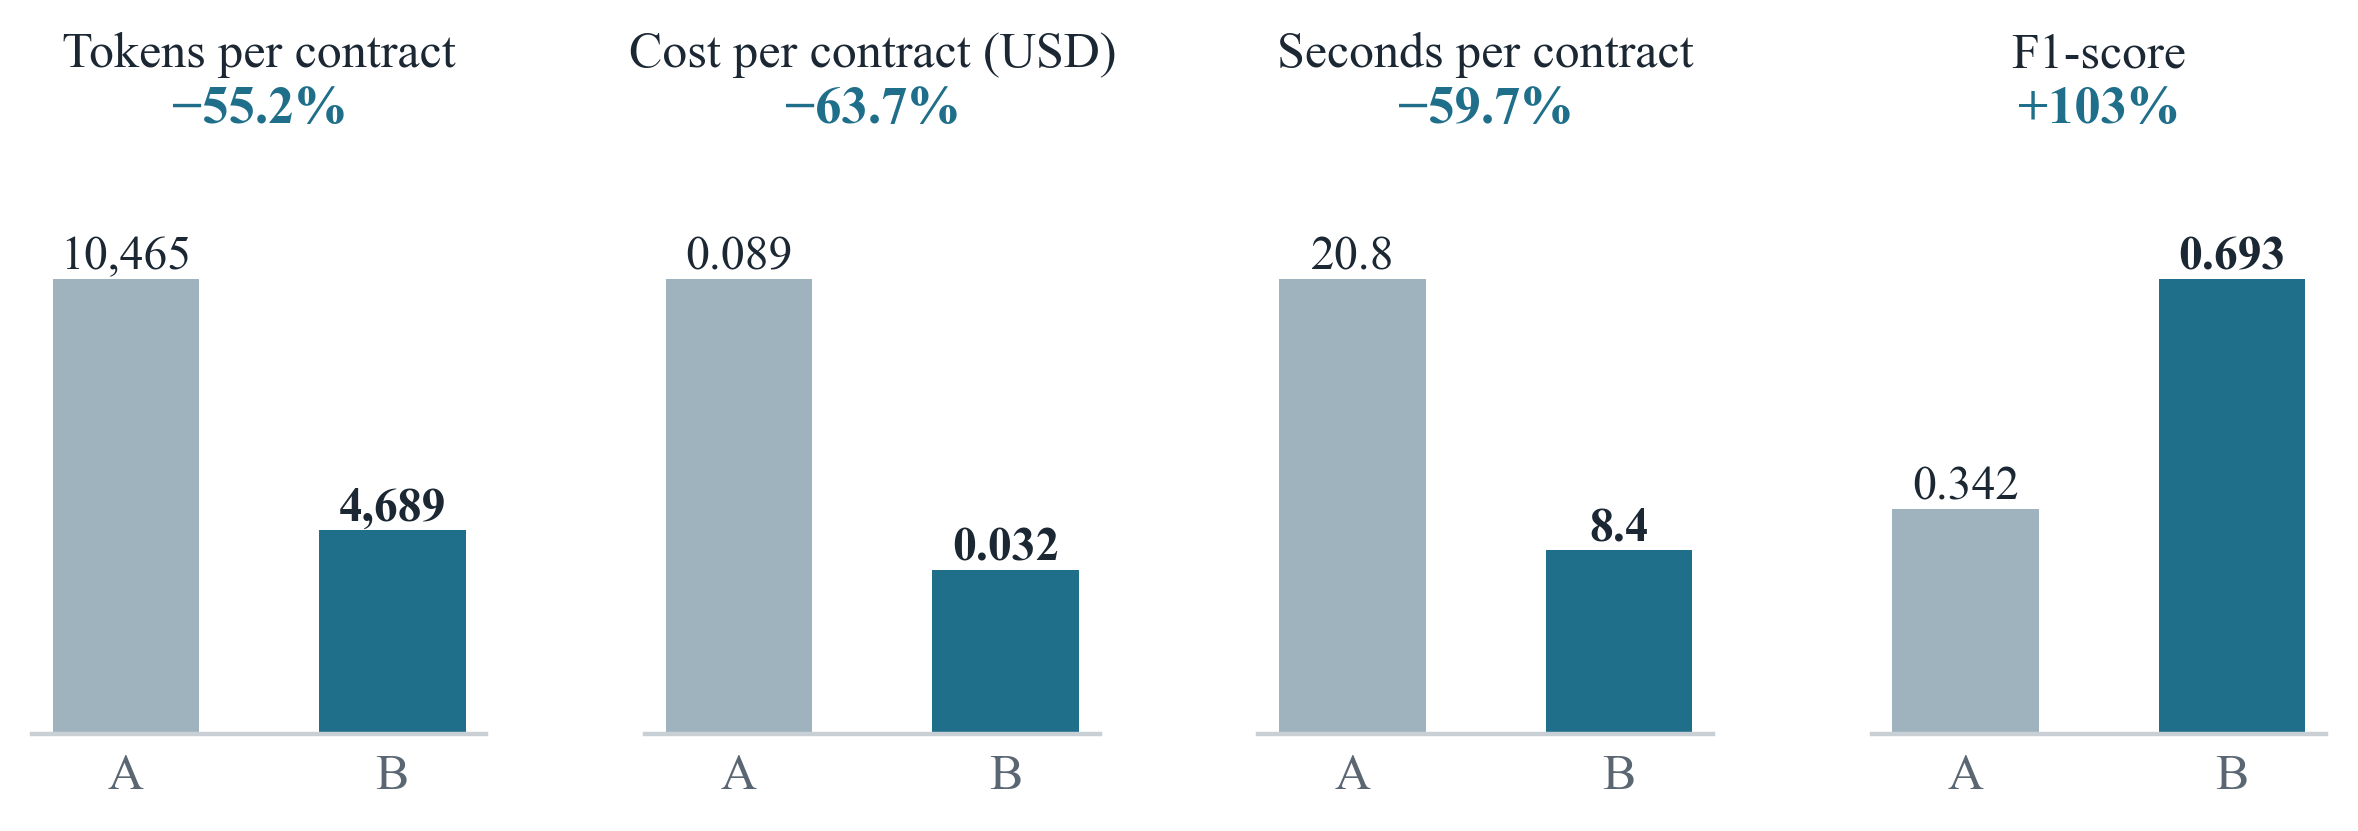
\includegraphics[width=0.92\linewidth, keepaspectratio]{fig3_resources.png}
    \caption{Resource use and detection quality per contract, Arm~A against Arm~B. Token consumption, cost and latency fall by more than half while F1-score doubles.}
    \label{fig:resources}
\end{figure*}

\subsection{Detection Effectiveness}\label{subsec:effectiveness}
Detection quality improved on every aggregate measure, as Table~\ref{tab:effectiveness} shows. Recall rose from 0.322 to 0.775 and precision from 0.365 to 0.627, so the additional detections were not obtained by indiscriminate over-reporting. F1-score improved from 0.342 to 0.693, Cohen's kappa from 0.097 to 0.549 and label agreement from 0.642 to 0.801. Twenty-eight contracts were classified correctly in all eight categories under the pipeline, against five under the practical baseline.

The confusion matrix locates the change. Missed vulnerabilities fell from 314 to 104 while false positives fell from 259 to 214, so both error types improved together and the result is not a threshold shift. At contract level, 142 contracts improved, 31 were unchanged and 27 regressed. Over the 1,600 paired cells, 170 were correct only under the baseline and 425 only under the pipeline, a two-sided McNemar exact $p$ of about $3.7 \times 10^{-26}$.

Two further measurements bound what may be attributed to each half of the treatment. First, the 130 contracts of the last sampling round were never inspected while the method was developed; on those alone the pipeline reaches an F1-score of 0.689 and an agreement of 0.797, against 0.340 and 0.634 for the baseline ($p \approx 4.1 \times 10^{-18}$), so the result is not an artefact of development on the evaluation set. Second, holding the prompt fixed and changing only the input, the slice neither improved nor degraded detection on a 70-contract subset (27 cells correct only with the complete source against 28 only with the slice, $p = 1.00$) while still reducing tokens. The accuracy reported here is therefore carried by the calibrated prompt and the token reduction by the slice; the contribution of this paper is that the two compose.

\begin{table}[t]
\centering
\caption{Detection Effectiveness Over 1,600 Label Cells}
\label{tab:effectiveness}
\footnotesize
\renewcommand{\arraystretch}{1.2}
\begin{tabular}{@{}l r r r@{}}
\hline
\textbf{Metric} & \textbf{Arm A} & \textbf{Arm B} & \textbf{Change} \\
\hline\hline
Label agreement & 0.642 & 0.801 & $+$0.159 \\
Hamming loss & 0.358 & 0.199 & $-$0.159 \\
Exact match (8/8) & 5/200 & 28/200 & $+$23 \\
Precision & 0.365 & 0.627 & $+$0.262 \\
Recall & 0.322 & 0.775 & $+$0.453 \\
F1-score & 0.342 & 0.693 & $+$0.351 \\
Cohen's kappa & 0.097 & 0.549 & $+$0.452 \\
True positives & 149 & 359 & $+$210 \\
False positives & 259 & 214 & $-$45 \\
False negatives & 314 & 104 & $-$210 \\
\hline
\end{tabular}
\end{table}

\subsection{Per-Category Behaviour}\label{subsec:percat}
Table~\ref{tab:percat} and Fig.~\ref{fig:percat} report every category. Six categories improve and two regress. The two largest movements are reentrancy, whose F1-score rises from 0.19 to 0.82 as missed vulnerabilities fall from 88 to 2, and access control, from 0.41 to 0.83 with misses falling from 102 to 9. Both are categories in which the practical baseline is conservative: asked to report only what is reachable and exploitable, the detector marked 10 of 98 reentrancy contracts and 42 of 144 access-control contracts, while the \texttt{MUTFN} anchor tags precisely the state-mutating entry points where a missing modifier would live. Unchecked return values improve from 0.46 to 0.74 and DoS from 0.17 to 0.47, in both cases by removing false positives rather than by finding more, and arithmetic and bad randomness improve modestly. The two regressions are instructive. Time manipulation falls from 0.67 to 0.58 because the calibrated rule recovers misses, from 15 to 4, at the cost of raising false positives from 11 to 50. Front running falls from 0.09 to 0.00: the rule suppresses the category so strongly that it cuts 132 false positives to 14 but recovers none of its 15 positives. That category is produced by a single analyser in the reference and carries no lexical signal a detector can act on, as Section~\ref{sec:limit} discusses.

\begin{table*}[htbp]
\centering
\caption{Per-Category Detection Detail Across All Eight DASP Categories}
\label{tab:percat}
\footnotesize
\renewcommand{\arraystretch}{1.2}
\begin{tabular}{l r r r r r r r}
\hline
\textbf{Category} & \textbf{DIVE +} & \textbf{Agreement (A)} & \textbf{Agreement (B)} & \textbf{F1 (A)} & \textbf{F1 (B)} & \textbf{FN (A)} & \textbf{FN (B)} \\
\hline\hline
Reentrancy & 98 & 0.560 & 0.795 & 0.19 & 0.82 & 88 & 2 \\
Access Control & 144 & 0.405 & 0.725 & 0.41 & 0.83 & 102 & 9 \\
Arithmetic & 84 & 0.610 & 0.570 & 0.44 & 0.52 & 53 & 38 \\
Unchecked Return Values & 38 & 0.785 & 0.910 & 0.46 & 0.74 & 20 & 13 \\
DoS & 26 & 0.655 & 0.875 & 0.17 & 0.47 & 19 & 15 \\
Bad Randomness & 16 & 0.950 & 0.950 & 0.58 & 0.62 & 9 & 8 \\
Front Running & 15 & 0.300 & 0.855 & 0.09 & 0.00 & 8 & 15 \\
Time manipulation & 42 & 0.870 & 0.730 & 0.67 & 0.58 & 15 & 4 \\
\hline
\textbf{All categories} & \textbf{463} & \textbf{0.642} & \textbf{0.801} & \textbf{0.342} & \textbf{0.693} & \textbf{314} & \textbf{104} \\
\hline
\multicolumn{8}{@{}p{16.5cm}@{}}{\scriptsize DIVE + counts reference positives. A is Arm~A, the complete source with the simple instruction; B is Arm~B, the AnchorSlice pipeline. FN counts missed vulnerabilities.} \\
\end{tabular}
\end{table*}

\begin{figure*}[t]
    \centering
    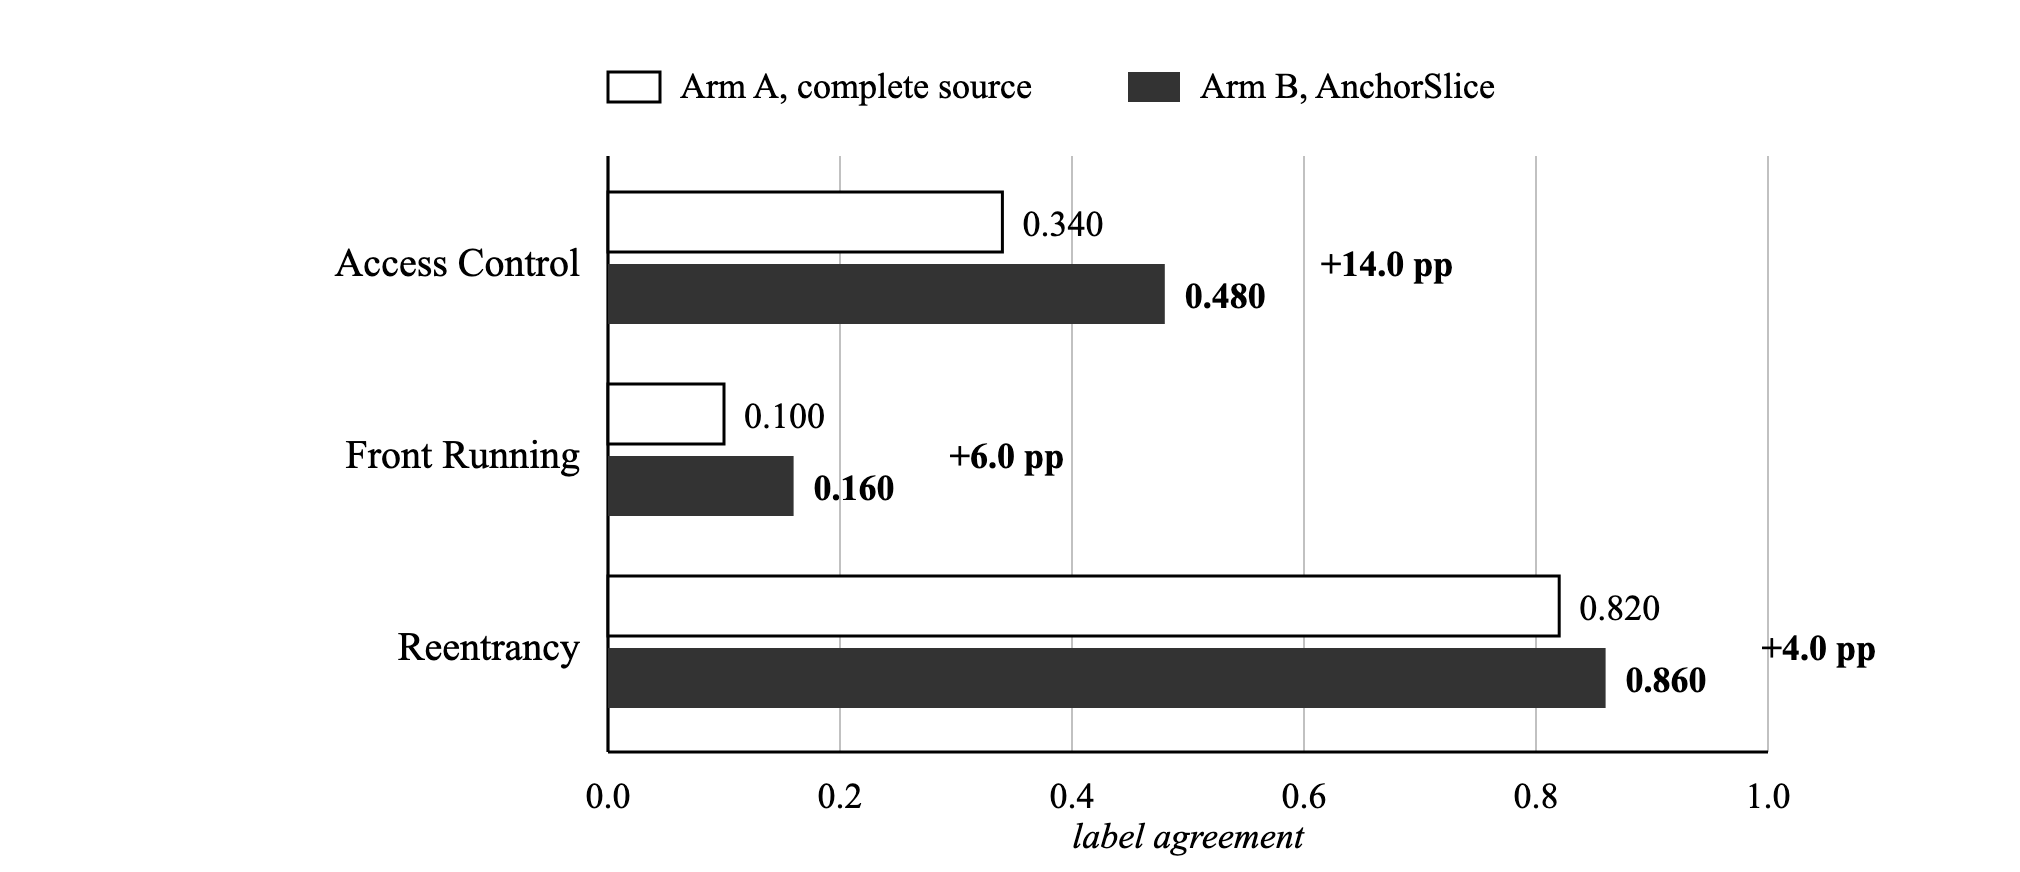
\includegraphics[width=\linewidth, keepaspectratio]{fig2_per_category.png}
    \caption{F1-score per DASP category for the two arms, ordered by the size of the change. Six categories improve under the pipeline; time manipulation and front running, drawn in the contrasting colour, regress.}
    \label{fig:percat}
\end{figure*}

\subsection{Discussion}\label{subsec:discussion}
The central observation is that discarding roughly 40\% of the source characters did not degrade the detector's judgement and, on aggregate measures, improved it. The simplest reading is that the removed text was not being used. Comment blocks, licence headers and unmodified library implementations carry no information on which a security judgement depends, and the detector appears to treat them accordingly. This is consistent with the observation that evidence buried inside long inputs is attended to less reliably than evidence near the edges~\cite{liu2024lost}: shortening the input raises the density of security-relevant material and shortens the distance between related fragments. The stage decomposition adds a second insight. Comment removal alone brings the corpus to 77.8\% of its original size and the remaining stages to 56.5\%, so removal accounts for most of the compression while the anchoring stage spends part of its saving on block headers. The value of anchoring therefore lies less in compression than in localisation: the tags tell the detector where each category could plausibly live, which suggests that an anchor is useful in proportion to how selective it is. The two categories whose tags are most selective, bad randomness and time manipulation at roughly one block in eight, are also the two the baseline already handled best, while the categories whose tags fire on more than half of all blocks are the ones where a calibrated decision rule, rather than the tag alone, carries the improvement.

\noindent We now revisit the three research questions raised in Section~\ref{sec:introduction}.

\noindent\textbf{RQ1 --- Evidence retention.}
AnchorSlice retained 56.5\% of the characters of the 200-contract sample, and every one of the 463 label-positive category instances kept at least one block tagged with its category, a retention of 1.00 in all eight categories. Comment removal and library collapse delivered most of the reduction; the rescue rule, together with guards for legacy visibility, multi-line signatures, anonymous fallbacks and minified sources, was necessary to reach full retention. The slicer needs no compilation and processes a contract in 7.6~ms on average.

\noindent\textbf{To best answer RQ1:}
A purely lexical, taxonomy-anchored slice can remove about two fifths of a contract's source while preserving evidence for every labelled vulnerability category in our sample, at a runtime cost that is negligible within a detection pipeline. Because retention is measured at contract level and the anchors were developed on the same sample, this result establishes that the slicer does not discard labelled evidence in-sample, not that it retains the specific vulnerable statements on unseen contracts.

\noindent\textbf{RQ2 --- Token efficiency.}
The pipeline reduced total token consumption by 55.2\%, from 10,465 to 4,689 tokens per contract, wall-clock detection time by 59.7\% and cost by 63.7\%, or \$0.032 against \$0.089 per contract. The contract text the detector reads fell by 69.1\%, and output tokens fell by 55.9\% because a compact, tagged input also shortens the detector's justifications.

\noindent\textbf{To best answer RQ2:}
AnchorSlice more than halves the token consumption of source-level vulnerability detection and shortens its runtime by about a fifth. Token count and latency are the portable benefits; the monetary saving depends on how a detector's pricing weights cached input against output and was small in our configuration.

\noindent\textbf{RQ3 --- Detection effectiveness.}
Recall rose from 0.322 to 0.775, precision from 0.365 to 0.627, F1-score from 0.342 to 0.693 and Cohen's kappa from 0.097 to 0.549, with missed vulnerabilities falling from 314 to 104 and false positives from 259 to 214. Six categories improved, most strongly reentrancy (F1-score 0.19 to 0.82) and access control (0.41 to 0.83); two regressed, time manipulation (0.67 to 0.58) and front running, which the calibrated rule suppresses so strongly that it recovers none of its 15 positives while cutting 132 false positives to 14. The paired McNemar test gives $p \approx 3.7 \times 10^{-26}$, and the 130 contracts never used in development give the same picture (F1-score 0.689).

\noindent\textbf{To best answer RQ3:}
Slicing did not harm vulnerability detection while more than halving token use, and it improved every aggregate effectiveness measure in our sample, driven by recovered false negatives in categories whose anchors are selective. Because the improvements are not statistically significant and each arm was run once, we read them as encouraging rather than established, and the firm conclusion is that taxonomy-aware input reduction is compatible with effective detection. The DoS result identifies anchor selectivity as the property to control in future versions of the slicer.

%============================================================
\section{Limitations and Threats to Validity}\label{sec:limit}
%============================================================
The results above come from one detector, one benchmark and a single run per arm, and several properties of the design and of the evaluation bound how far they generalise. This section states these limits explicitly so that the reported numbers are interpreted within them. It first addresses the strength of the detection results and the gap between token and monetary savings, then two design issues exposed by the per-category analysis, and finally threats arising from how evidence retention was validated, from the sample, and from the detector used.

\noindent\emph{What the treatment combines.} Arm~B changes both the detector's input and its prompt, so the headline comparison measures the pipeline as a whole against ordinary practice rather than the slice in isolation. The two components were separated on a 70-contract subset: with the prompt held fixed, the slice left detection unchanged ($p = 1.00$) while reducing tokens, so the token savings are attributable to the slice and the accuracy to the calibrated prompt. A tag-free slice arm would further separate the effect of removing code from that of naming candidate categories.

\noindent\emph{Portability of the cost figure.} Cost fell slightly faster than token count because the removed tokens are input rather than output. Detectors whose pricing weights these classes differently, or that bill cached input at a different rate, will see a different monetary figure, so token count and latency are the more portable benefits.

\noindent\emph{Two categories the pipeline does not solve.} Front running is the clearest failure: Arm~B marks none of its 15 positives, trading the baseline's 132 false positives for 14 at the cost of every true detection. In the reference, that category is produced by a single analyser, and no lexical pattern we measured predicts it: the ERC-20 approve allowance race, the textbook shape, appears in 164 of the 200 contracts and predicts the label with a precision of 0.04. Time manipulation moves the other way, recovering misses at the cost of raising false positives from 11 to 50. Relatedly, library collapse identifies constructs by name, so a contract that reuses a standard name for a modified implementation would have that code collapsed as well.

\noindent\emph{Confounded treatment.} Arm~B both removes code and adds category tags, and the DoS result suggests that these two changes can act in opposite directions, so the aggregate outcome may understate the benefit of removal alone. A tag-free arm is needed to separate them.

\noindent\emph{Weak retention criterion.} DIVE labels contracts rather than lines, so evidence retention of 1.00 means only that a positive contract keeps some block tagged with that category, not that it keeps the specific statements an annotator had in mind. The DIVE labels are themselves derived from a consensus of static analysers with post-hoc validation, so effectiveness is measured against the benchmark's annotation policy rather than against audited ground truth.

\noindent\emph{Development set and run-to-run variation.} The anchors and the calibrated decision rules were developed against a subset of the corpus, so figures over the whole sample are in part an in-sample fit; we therefore also report the 130 contracts of the final sampling round, which were never inspected during development and on which the result is unchanged. Each arm was run once. Three repetitions of one configuration on a fixed subset varied by 4.2 percentage points of agreement, which bounds the noise in single-run comparisons and is an order of magnitude smaller than the effect reported here.

\noindent\emph{One detector, one benchmark.} Both arms use a single proprietary model accessed through an interface that does not expose sampling parameters or allow a dated model snapshot to be pinned. Although the slice is detector-agnostic by construction, its effect on other source-level detectors, including open-weight models and multi-stage pipelines such as LineGuard~\cite{lineguard}, has not been measured. The evaluation also uses one benchmark whose labels are the union of six analysers, so agreement measures reproduction of a tool consensus rather than of audited ground truth, and the calibrated decision rules follow that consensus rather than Solidity semantics alone.

%============================================================
\section{Conclusion and Future Work}\label{sec:conclusion}
%============================================================
This paper addressed the token cost of smart contract vulnerability detection and showed that a large share of that cost can be removed before the detector runs. We presented AnchorSlice, a static slicing stage that reduces a Solidity contract to the fragments capable of hosting each DASP category, and evaluated it on the DIVE benchmark by changing only the detector's input. This section summarises the findings and the directions they open.

AnchorSlice is lexical throughout, needs no compilation, and processes a contract in 7.6~ms on average. On 200 contracts it retained evidence for all 463 labelled category instances, a retention of 1.00 in every category, while emitting 56.5\% of the original characters. Against the way such a detector is used in practice, the pipeline reduced token consumption by 55.2\%, cost by 63.7\% and runtime by 59.7\%, while raising F1-score from 0.342 to 0.693, agreement from 0.642 to 0.801 and Cohen's kappa from 0.097 to 0.549, cutting missed vulnerabilities from 314 to 104 and false positives from 259 to 214 at the same time ($p \approx 3.7 \times 10^{-26}$, and F1-score 0.689 on the 130 contracts never used in development). Token cost and detection quality therefore improve together: the saving comes from the slice and the accuracy from the calibrated prompt, and the two compose.

Four directions follow. A tag-free arm would separate the effect of removing code from the effect of naming candidate categories, and would also remove the header overhead that currently offsets the anchoring stage. A selectivity threshold that suppresses any category tagging more than a set fraction of a contract's blocks would address the DoS failure directly while preserving the access-control gain. The anchors should be re-validated on a held-out DIVE split, with the protocol repeated across several runs, before the approach is applied to the full corpus. Finally, the slice should be evaluated in front of other detectors, including open-weight models and our LineGuard framework, to establish that the token savings transfer across detection architectures.

\section{Disclosure Statement}
The authors declare that they have no relevant or material financial interests related to the research described in this paper.

%============================================================
\begin{thebibliography}{00}
%============================================================

\bibitem{szabo1997}
Szabo, N.: `Formalizing and Securing Relationships on Public Networks', \textit{First Monday}, 1997, 2, (9), doi: \href{https://doi.org/10.5210/fm.v2i9.548}{10.5210/fm.v2i9.548}

\bibitem{wood2014}
Wood, G.: `Ethereum: A Secure Decentralised Generalised Transaction Ledger', \textit{Ethereum Project Yellow Paper}, 2014, \url{https://ethereum.github.io/yellowpaper/paper.pdf}

\bibitem{luu2016}
Luu, L., Chu, D.-H., Olickel, H., Saxena, P., Hobor, A.: `Making Smart Contracts Smarter'. \textit{Proc. ACM SIGSAC Conf. Computer and Communications Security (CCS)}, 2016, pp. 254--269, doi: \href{https://doi.org/10.1145/2976749.2978309}{10.1145/2976749.2978309}

\bibitem{dasp}
NCC Group: `Decentralized Application Security Project (DASP) Top 10', 2018, \url{https://dasp.co}

\bibitem{durieux2020}
Durieux, T., Ferreira, J.F., Abreu, R., Cruz, P.: `Empirical Review of Automated Analysis Tools on 47,587 Ethereum Smart Contracts'. \textit{Proc. ACM/IEEE Int. Conf. Software Engineering (ICSE)}, 2020, pp. 530--541, doi: \href{https://doi.org/10.1145/3377811.3380364}{10.1145/3377811.3380364}

\bibitem{ghaleb2020}
Ghaleb, A., Pattabiraman, K.: `How Effective Are Smart Contract Analysis Tools? Evaluating Smart Contract Static Analysis Tools Using Bug Injection'. \textit{Proc. ACM SIGSOFT Int. Symp. Software Testing and Analysis (ISSTA)}, 2020, pp. 415--427, doi: \href{https://doi.org/10.1145/3395363.3397385}{10.1145/3395363.3397385}

\bibitem{feist2019}
Feist, J., Grieco, G., Groce, A.: `Slither: A Static Analysis Framework for Smart Contracts'. \textit{Proc. IEEE/ACM Int. Workshop on Emerging Trends in Software Engineering for Blockchain (WETSEB)}, 2019, pp. 8--15, doi: \href{https://doi.org/10.1109/WETSEB.2019.00008}{10.1109/WETSEB.2019.00008}

\bibitem{zhuang2020}
Zhuang, Y., Liu, Z., Qian, P., Liu, Q., Wang, X., He, Q.: `Smart Contract Vulnerability Detection Using Graph Neural Network'. \textit{Proc. Int. Joint Conf. Artificial Intelligence (IJCAI)}, 2020, pp. 3283--3290, doi: \href{https://doi.org/10.24963/ijcai.2020/454}{10.24963/ijcai.2020/454}

\bibitem{sun2024gptscan}
Sun, Y., Wu, D., Xue, Y., Liu, H., Wang, H., Xu, Z., Xie, X., Liu, Y.: `GPTScan: Detecting Logic Vulnerabilities in Smart Contracts by Combining GPT with Program Analysis'. \textit{Proc. IEEE/ACM Int. Conf. Software Engineering (ICSE)}, 2024, pp. 1--13, doi: \href{https://doi.org/10.1145/3597503.3639117}{10.1145/3597503.3639117}

\bibitem{hu2023gptlens}
Hu, S., Huang, T., \.{I}lhan, F., Tekin, S.F., Liu, L.: `Large Language Model-Powered Smart Contract Vulnerability Detection: New Perspectives'. \textit{Proc. IEEE Int. Conf. Trust, Privacy and Security in Intelligent Systems and Applications (TPS-ISA)}, 2023, pp. 297--306, doi: \href{https://doi.org/10.1109/TPS-ISA58951.2023.00044}{10.1109/TPS-ISA58951.2023.00044}

\bibitem{ma2025iaudit}
Ma, W., Wu, D., Sun, Y., Wang, T., Liu, S., Zhang, J., Xue, Y., Liu, Y.: `Combining Fine-Tuning and LLM-Based Agents for Intuitive Smart Contract Auditing with Justifications'. \textit{Proc. IEEE/ACM Int. Conf. Software Engineering (ICSE)}, 2025, pp. 1--13, \href{https://arxiv.org/abs/2403.16073}{arXiv:2403.16073}

\bibitem{he2024review}
He, Z., Li, Z., Yang, S., Qiao, A., Zhang, X., Luo, X., Chen, T.: `Large Language Models for Blockchain Security: A Systematic Literature Review', \textit{arXiv preprint}, 2024, \href{https://arxiv.org/abs/2403.14280}{arXiv:2403.14280}

\bibitem{liu2024lost}
Liu, N.F., Lin, K., Hewitt, J., Paranjape, A., Bevilacqua, M., Petroni, F., Liang, P.: `Lost in the Middle: How Language Models Use Long Contexts', \textit{Trans. Assoc. Computational Linguistics}, 2024, 12, pp. 157--173, doi: \href{https://doi.org/10.1162/tacl_a_00638}{10.1162/tacl\_a\_00638}

\bibitem{jiang2023llmlingua}
Jiang, H., Wu, Q., Lin, C.-Y., Yang, Y., Qiu, L.: `LLMLingua: Compressing Prompts for Accelerated Inference of Large Language Models'. \textit{Proc. Conf. Empirical Methods in Natural Language Processing (EMNLP)}, 2023, pp. 13358--13376, doi: \href{https://doi.org/10.18653/v1/2023.emnlp-main.825}{10.18653/v1/2023.emnlp-main.825}

\bibitem{weiser1981}
Weiser, M.: `Program Slicing'. \textit{Proc. Int. Conf. Software Engineering (ICSE)}, 1981, pp. 439--449, \url{https://dl.acm.org/doi/10.5555/800078.802557}

\bibitem{lineguard}
Pakshad, P., Aghanasiri, S., Shameli-Sendi, A., Omar, M.: `LineGuard: An LLM-Based Smart Contract Vulnerability Detection', manuscript under review, 2025, \url{https://github.com/sjag77/LineGuard}

\bibitem{dive2026}
Alsunaidi, S.J., Aljamaan, H., Hammoudeh, M.: `DIVE: A Multi-Label Smart Contract Vulnerability Dataset', \textit{Scientific Data}, 2026, 13, art. 664; dataset: \href{https://doi.org/10.5281/zenodo.18519253}{10.5281/zenodo.18519253}

\bibitem{tsankov2018}
Tsankov, P., Dan, A., Drachsler-Cohen, D., Gervais, A., B\"{u}nzli, F., Vechev, M.: `Securify: Practical Security Analysis of Smart Contracts'. \textit{Proc. ACM SIGSAC Conf. Computer and Communications Security (CCS)}, 2018, pp. 67--82, doi: \href{https://doi.org/10.1145/3243734.3243780}{10.1145/3243734.3243780}

\bibitem{tikhomirov2018}
Tikhomirov, S., Voskresenskaya, E., Ivanitskiy, I., Takhaviev, R., Marchenko, E., Alexandrov, Y.: `SmartCheck: Static Analysis of Ethereum Smart Contracts'. \textit{Proc. IEEE/ACM Int. Workshop on Emerging Trends in Software Engineering for Blockchain (WETSEB)}, 2018, pp. 9--16, doi: \href{https://doi.org/10.1145/3194113.3194115}{10.1145/3194113.3194115}

\bibitem{mythril}
ConsenSys: `Mythril: Security Analysis Tool for EVM Bytecode', 2018, \url{https://github.com/ConsenSys/mythril}

\bibitem{nikolic2018}
Nikoli\'{c}, I., Kolluri, A., Sergey, I., Saxena, P., Hobor, A.: `Finding the Greedy, Prodigal, and Suicidal Contracts at Scale'. \textit{Proc. Annual Computer Security Applications Conf. (ACSAC)}, 2018, pp. 653--663, doi: \href{https://doi.org/10.1145/3274694.3274743}{10.1145/3274694.3274743}

\bibitem{so2020}
So, S., Lee, M., Park, J., Lee, H., Oh, H.: `VeriSmart: A Highly Precise Safety Verifier for Ethereum Smart Contracts'. \textit{Proc. IEEE Symp. Security and Privacy (S\&P)}, 2020, pp. 1678--1694, doi: \href{https://doi.org/10.1109/SP40000.2020.00032}{10.1109/SP40000.2020.00032}

\bibitem{jiang2018contractfuzzer}
Jiang, B., Liu, Y., Chan, W.K.: `ContractFuzzer: Fuzzing Smart Contracts for Vulnerability Detection'. \textit{Proc. ACM/IEEE Int. Conf. Automated Software Engineering (ASE)}, 2018, pp. 259--269, doi: \href{https://doi.org/10.1145/3238147.3238177}{10.1145/3238147.3238177}

\bibitem{nguyen2020sfuzz}
Nguyen, T.D., Pham, L.H., Sun, J., Lin, Y., Minh, Q.T.: `sFuzz: An Efficient Adaptive Fuzzer for Solidity Smart Contracts'. \textit{Proc. ACM/IEEE Int. Conf. Software Engineering (ICSE)}, 2020, pp. 778--788, doi: \href{https://doi.org/10.1145/3377811.3380334}{10.1145/3377811.3380334}

\bibitem{li2018vuldeepecker}
Li, Z., Zou, D., Xu, S., Ou, X., Jin, H., Wang, S., Deng, Z., Zhong, Y.: `VulDeePecker: A Deep Learning-Based System for Vulnerability Detection'. \textit{Proc. Network and Distributed System Security Symp. (NDSS)}, 2018, doi: \href{https://doi.org/10.14722/ndss.2018.23158}{10.14722/ndss.2018.23158}

\bibitem{li2022sysevr}
Li, Z., Zou, D., Xu, S., Jin, H., Zhu, Y., Chen, Z.: `SySeVR: A Framework for Using Deep Learning to Detect Software Vulnerabilities', \textit{IEEE Trans. Dependable and Secure Computing}, 2022, 19, (4), pp. 2244--2258, doi: \href{https://doi.org/10.1109/TDSC.2021.3051525}{10.1109/TDSC.2021.3051525}

\bibitem{zhou2019devign}
Zhou, Y., Liu, S., Siow, J., Du, X., Liu, Y.: `Devign: Effective Vulnerability Identification by Learning Comprehensive Program Semantics via Graph Neural Networks'. \textit{Proc. Advances in Neural Information Processing Systems (NeurIPS)}, 2019, pp. 10197--10207, \href{https://arxiv.org/abs/1909.03496}{arXiv:1909.03496}

\bibitem{fu2022linevul}
Fu, M., Tantithamthavorn, C.: `LineVul: A Transformer-Based Line-Level Vulnerability Prediction'. \textit{Proc. IEEE/ACM Int. Conf. Mining Software Repositories (MSR)}, 2022, pp. 608--620, doi: \href{https://doi.org/10.1145/3524842.3528452}{10.1145/3524842.3528452}

\bibitem{feng2020codebert}
Feng, Z., Guo, D., Tang, D., Duan, N., Feng, X., Gong, M., Shou, L., Qin, B., Liu, T., Jiang, D., Zhou, M.: `CodeBERT: A Pre-Trained Model for Programming and Natural Languages'. \textit{Findings of the Association for Computational Linguistics: EMNLP}, 2020, pp. 1536--1547, doi: \href{https://doi.org/10.18653/v1/2020.findings-emnlp.139}{10.18653/v1/2020.findings-emnlp.139}

\bibitem{liu2023combining}
Liu, Z., Qian, P., Wang, X., Zhuang, Y., Qiu, L., Wang, X.: `Combining Graph Neural Networks with Expert Knowledge for Smart Contract Vulnerability Detection', \textit{IEEE Trans. Knowledge and Data Engineering}, 2023, 35, (2), pp. 1296--1310, doi: \href{https://doi.org/10.1109/TKDE.2021.3095196}{10.1109/TKDE.2021.3095196}

\bibitem{chen2021codex}
Chen, M., et al.: `Evaluating Large Language Models Trained on Code', \textit{arXiv preprint}, 2021, \href{https://arxiv.org/abs/2107.03374}{arXiv:2107.03374}

\bibitem{brown2020}
Brown, T.B., et al.: `Language Models Are Few-Shot Learners'. \textit{Proc. Advances in Neural Information Processing Systems (NeurIPS)}, 2020, pp. 1877--1901, \href{https://arxiv.org/abs/2005.14165}{arXiv:2005.14165}

\bibitem{wei2022cot}
Wei, J., Wang, X., Schuurmans, D., Bosma, M., Ichter, B., Xia, F., Chi, E., Le, Q., Zhou, D.: `Chain-of-Thought Prompting Elicits Reasoning in Large Language Models'. \textit{Proc. Advances in Neural Information Processing Systems (NeurIPS)}, 2022, pp. 24824--24837, \href{https://arxiv.org/abs/2201.11903}{arXiv:2201.11903}

\bibitem{sun2024llm4vuln}
Sun, Y., Wu, D., Xue, Y., Liu, H., Ma, W., Zhang, L., Shi, M., Liu, Y.: `LLM4Vuln: A Unified Evaluation Framework for Decoupling and Enhancing LLMs' Vulnerability Reasoning', \textit{arXiv preprint}, 2024, \href{https://arxiv.org/abs/2401.16185}{arXiv:2401.16185}

\bibitem{wei2024smartaudit}
Wei, Z., Sun, J., Zhang, Z., Zhang, X., Yang, X., Zhu, L.: `LLM-SmartAudit: Advanced Smart Contract Vulnerability Detection', \textit{arXiv preprint}, 2024, \href{https://arxiv.org/abs/2410.09381}{arXiv:2410.09381}

\bibitem{yu2024smartllama}
Yu, L., Chen, S., Yuan, H., Wang, P., Huang, Z., Zhang, J., Shen, C., Zhang, F., Yang, J., Li, J.: `Smart-LLaMA: Two-Stage Post-Training of Large Language Models for Smart Contract Vulnerability Detection and Explanation', \textit{arXiv preprint}, 2024, \href{https://arxiv.org/abs/2411.06221}{arXiv:2411.06221}

\bibitem{liu2025propertygpt}
Liu, Y., Xue, Y., Wu, D., Sun, Y., Li, Y., Shi, M., Liu, Y.: `PropertyGPT: LLM-Driven Formal Verification of Smart Contracts Through Retrieval-Augmented Property Generation'. \textit{Proc. Network and Distributed System Security Symp. (NDSS)}, 2025, doi: \href{https://doi.org/10.14722/ndss.2025.241357}{10.14722/ndss.2025.241357}

\bibitem{jiang2024longllmlingua}
Jiang, H., Wu, Q., Luo, X., Li, D., Lin, C.-Y., Yang, Y., Qiu, L.: `LongLLMLingua: Accelerating and Enhancing LLMs in Long Context Scenarios via Prompt Compression'. \textit{Proc. Annual Meeting of the Association for Computational Linguistics (ACL)}, 2024, pp. 1658--1677, doi: \href{https://doi.org/10.18653/v1/2024.acl-long.91}{10.18653/v1/2024.acl-long.91}

\bibitem{lewis2020rag}
Lewis, P., et al.: `Retrieval-Augmented Generation for Knowledge-Intensive NLP Tasks'. \textit{Proc. Advances in Neural Information Processing Systems (NeurIPS)}, 2020, pp. 9459--9474, \href{https://arxiv.org/abs/2005.11401}{arXiv:2005.11401}

\bibitem{sridharan2007}
Sridharan, M., Fink, S.J., Bod\'{\i}k, R.: `Thin Slicing'. \textit{Proc. ACM SIGPLAN Conf. Programming Language Design and Implementation (PLDI)}, 2007, pp. 112--122, doi: \href{https://doi.org/10.1145/1250734.1250748}{10.1145/1250734.1250748}

\bibitem{yashavant2022}
Yashavant, C.S., Kumar, S., Karkare, A.: `ScrawlD: A Dataset of Real World Ethereum Smart Contracts Labelled with Vulnerabilities', \textit{arXiv preprint}, 2022, \href{https://arxiv.org/abs/2202.11409}{arXiv:2202.11409}

\bibitem{zheng2024dappscan}
Zheng, Z., Su, J., Chen, J., Lo, D., Zhong, Z., Ye, M.: `DAppSCAN: Building Large-Scale Datasets for Smart Contract Weaknesses in DApp Projects', \textit{IEEE Trans. Software Engineering}, 2024, 50, (6), pp. 1360--1373, doi: \href{https://doi.org/10.1109/TSE.2024.3383422}{10.1109/TSE.2024.3383422}

\bibitem{anchorslice_repo}
Repository available at \url{https://github.com/sjag77/AnchorSlice}

\end{thebibliography}

\vspace{-34pt}

\begin{IEEEbiography}[{
\includegraphics[width=1in,height=1.25in,clip,keepaspectratio]{sajad.jpg}}]{SAJAD AGHANASIRI} is currently an M.Sc. student in Software Engineering at Shahid Beheshti University (SBU), Tehran, Iran. He received his B.Sc. in Computer Engineering from Islamic Azad University, Central Tehran Branch (IAU-CTB). His thesis focuses on securing smart contracts via vulnerability detection in code snippets and program analysis, exploring static, semantic, and hybrid techniques. His research interests span software security, blockchain/smart-contract security, program analysis, and complex networks. He has served as a Teaching Assistant for one academic term.
\end{IEEEbiography}

\vspace{-0.9cm}

\begin{IEEEbiography}[{
\includegraphics[width=1in,height=1.25in,clip,keepaspectratio]{sina.jpg}}]{SINA ZAKER} is currently an M.Sc. student in Network Security at Shahid Beheshti University (SBU), Tehran, Iran. He received his B.Sc. in Computer Engineering. His thesis focuses on defending Graph Neural Networks (GNNs) against structural adversarial attacks, exploring robust mitigation strategies and adaptive spectral filtering models. His primary research interests span network security, artificial intelligence security, Web Application Firewalls (WAF), complex graphs, adversarial machine learning, and the security of distributed cloud systems.
\end{IEEEbiography}

\vspace{-0.9cm}

\begin{IEEEbiography}[{
\includegraphics[width=1in,height=1.25in,clip,keepaspectratio]{shameli.jpg}}]{ALIREZA SHAMELI-SENDI} is currently an Associate Professor at Shahid Beheshti University. Before joining SBU, he was a Postdoctoral Fellow at Ericsson, Canada and Postdoctoral at ETS and McGill universities in collaboration with Ericsson. He received his Ph.D degree in computer engineering from Montreal University (Ecole Polytechnique de Montreal), Canada. He obtained his B.Sc. and M.Sc. from Amirkabir University of Technology. His primary research interests include information security, intrusion response system, and cloud computing. He is a recipient of Postdoctoral Research Fellowship Award and Industrial Postdoctoral Fellowship Award from Canada. In addition, he received the best researcher awards, at SBU, in 2018 and 2022.
\end{IEEEbiography}

\EOD

\end{document}
